\chapter{Datastream Extraction Tool} \label{chapter:datastream-extraction-tool}
Various algorithms have been developed to compute the skyline of a given set of tuples. To date, no multipurpose skyline algorithm exists that would perform equally well in every environment and under any circumstances. Therefore, a number of algorithms have recently emerged that are each tailored to some very specific range of skyline problems. In this chapter, some of the most relevant up-to-date skyline algorithms are briefly introduced and the necessary theoretical foundation to the term skyline is given. 

\section{The Skyline Operator} \label{section:skyline-operator}
From a theoretical point of view, computing the skyline of a set of tuples corresponds to the mathematical problem of finding the maxima of a set of vectors~\cite{kung}. While the problem has been extensively described and analyzed by Kung et al. as early as in 1975~\cite{kung}, the term skyline in the context of databases was first introduced by D. Kossmann et al. in 2001~\cite{kossmann}, along with the first efficient skyline algorithms. 

The skyline of a set of tuples is defined as those tuples that are not dominated by any other tuple in the set. A tuple $p$ dominates a tuple $q$ if $p$ is not worse than $q$ in every given dimension and is better than $q$ in at least one dimension. Or, equally, 
\begin{equation}
p \succ q := \nexists i \in N^{+}_{0} . p[A_{i}] > q[A_{i}] \wedge \exists j \in N^{+}_{0} . p[A_{j}] < q[A_{j}]. 
\end{equation}
The definition assumes that the tuple attributes in each dimension have to be minimized. If they have to be maximized instead, then the $>$ and $<$ signs have to be flipped respectively. The notation $p[A_{i}]$ (resp. $q[A_{i}]$) stands for $p$'s (resp. $q$'s) $i$-th attribute value. 

%The process of computing the skyline of a range of tuples is visualized in Fig.~\ref{fig:skyline-example} for the apartment example. 



% maybe add that skyline operation is related to top-k queries etc. 

To integrate the operation of skyline computation into a database system was first proposed by Kossmann et al.~\cite{kossmann} in 2001. The researchers suggested a skyline extension to SQL that would filter out the tuples from the underlying database that are not worse than any other tuple. The SQL syntax proposed to be incorporated into the structure of a query would be similar to: 
\begin{minted}{sql}
SELECT ... FROM ... WHERE ...
GROUP BY ... HAVING ...
SKYLINE OF [DISTINCT] d1 [MIN | MAX], ... , dn [MIN | MAX]
ORDER BY ...
\end{minted}
Herein, $d_{1}$, ... , $d_{n}$ are the dimensions of the skyline. The annotations $MIN$ and $MAX$ specify for each dimension whether it has to be minimized or maximized. 
The authors argue that implementing the functionality of the skyline operator on top of the database is both costly and inefficient, and thus propose the new operator to be integrated directly into the database. 

\section{Database Context} \label{section:database-context}
The implementation of the skyline operator inside a database system is influenced by several, sometimes contradictory, criteria. These are, among others, the type of the database, its estimated size, the prevalent data types used, the requirements regarding time and resource usage, as well as the particular use cases in mind at the time of database design. 

% existence of an index, possibility of parallelization, cpu processing power, available main memory, communication with disc required or not 
One of the most common optimization approaches is to reduce the number of needed dominance checks, in order to compute the skyline with a lesser number of comparisons. This way, the CPU cost of the skyline operation can be significantly reduced. Therefore, this optimization technique is most sensible for database systems with generally limited computation resources. One of the algorithms taking this path of optimization is the ST-S algorithm \cite{rahman}, which will be discussed later in greater detail. 
The main drawback of such algorithms is generally higher memory usage, as the number of dominance checks is most easily reduced by using an extra data structure to ''sift'' the tuples through it. In most cases, this is some specially fitted form of tree which enables a significant reduction in tuple comparisons. This is why only database systems with a sufficient amount of main memory available at runtime are eligible for this type of optimization. For this reason, in-memory databases seem optimally fitted for such algorithms. 

Another criterion to account for is the estimated size of the original dataset. While some algorithms show excellent running times on low numbers of tuples, their runtime grows exponentially with the rising size of the input. Other algorithms, however, are best suited for very large datasets, usually by enabling various parallelization approaches. Large multicore database systems, specially optimized for computation-intensive OLAP queries are the best prerequisite for such algorithms. Some of the approaches are based on the well-known divide-and-conquer principle to achieve this goal. 

For database systems with frequent background storage access, a different optimization technique has been developed. In order to conduct the entire computation process within the (often limited) main memory, the tuples for the computation are always loaded block-wise, and the number of I/O accesses to the background storage is thus reduced. Block-Nested-Loops~\cite{kossmann} is one the most basic, but nonetheless efficient algorithms for this purpose. 

Depending on the data type of the attribute values stored in the tuples, some algorithms might prove not eligible for the particular scenario at all. This is for instance the case with tree-based algorithms where each attribute can only assume categorical values. The reason for this is that each node can maximally have as many child nodes as there are allowed attribute values. While this is usually not a problem for some bounded number of integer values, there are simply too many possible double values between any two range boundaries to create a new child node for each of them. 

%In addition to that, whenever an index structure exists on the tuples of the database, it can also be used to improve the performance of the skyline operation. Some of the algorithms taking this path will be further discussed in related work (section~\ref{section:related-work}). %are NN~\cite{nn} and BBS~\cite{bbs}, both based on Nearest-Neighbor-Search.

In the following and throughout this paper, a hybrid main-memory database system, such as HyPer~\cite{hyper}, is assumed as the context of this work. It combines the advantages of both OLTP and OLAP databases in one, and thus enables most of the optimization techniques mentioned above. While optimization approaches such as bulk-loading of the tuples into main memory are no longer required, improvements like tree-based dominance tests and also parallelization become possible. 

\section{Related Work} \label{section:related-work}
While a lot of work has been done developing high-performing algorithms for skyline computation, many aspects of the field are still not entirely covered. Such aspects include memory efficiency for progressive skyline algorithms, as well as parallelization of originally sequential approaches. The following section gives an overview of some of the most prominent skyline algorithms to date. 

\subsection{Naive-Nested-Loops Algorithm} \label{subsection:naive-nested-loops}
Arguably the simplest existing skyline algorithm is Naive-Nested-Loops. As mentioned by Kossmann et al, ``[t]his is essentially what happens if a Skyline query is implemented on top of a database system''\cite{kossmann}. 

The main idea behind the algorithm is to compare each tuple of the dataset with every other tuple. This is accomplished by creating two loops, one of them nested in the other, and for each tuple to traverse the entire dataset from beginning to end, in order to check whether the tuple is dominated by any other. If it is not dominated, then it is added to the resulting skyline. While Naive-Nested-Loops is very versatile and can be applied to almost every given dataset, it tends to perform badly in comparison to some of the newer algorithms. A pseudo-code notation of the algorithm is shown in Algorithm \ref{alg:nnl}. 

% pseudo-code Naive Nested-Loops
\begin{algorithm}[h]
	\caption{Naive Nested-Loops Algorithm} \label{alg:nnl}
	\begin{algorithmic}[1] 
		\State \textbf{Input :} Tuple List $T$
		\State \textbf{Output :} Skyline $skyline$
		\For {each tuple $t~\in~T$}
			\State $is\_not\_dominated \gets $True
			\For {each tuple $d~\in~T\backslash\{t\}$}
				\If {dominates($d$, $t$)}
					\State $is\_not\_dominated \gets $False
					\State Exit inner loop
				\EndIf
			\EndFor
			\If {$is\_not\_dominated$}
				\State Add $t$ to $skyline$
			\EndIf
		\EndFor
	\end{algorithmic}
\end{algorithm}

\subsection{Block-Nested-Loops Algorithm} \label{subsection:bnl}
One of the most basic skyline algorithms, and yet fairly efficient, is the Block-Nested-Loops~\cite{kossmann} algorithm (in the following BNL). It takes the concept of Naive-Nested-Loops and extends it by making sure that incomparable tuples are kept in a persisting \textit{window} in main memory. The main idea behind this is to reduce the number of necessary I/O operations when working with traditional DBMS, as disc storage has significantly longer access times than main memory~\cite{book-kemper}. 

Whenever a new tuple is inserted into the window, it is iteratively compared to all the other tuples that already find themselves in the window. At this point, one of the following happens: 
\begin{itemize}
	\item If the new tuple is dominated by some other tuple in the window, then it is eliminated and is no longer considered for the skyline. 
	\item If the new tuple dominates one or more of the other tuples in the window, then these tuples are eliminated from the window and are no longer considered for the skyline. The new tuple gets inserted into the window as a new skyline candidate. 
	\item If the new tuple is incomparable with all the other tuples in the window and there is enough space left in it, then it gets inserted. If there is not enough space in the window, then the new tuple is written to the temporary file on disc and will be considered again for further iterations of the algorithm. The last step with the temporary file is not necessary if a main memory database is used, because in this case all the incomparable tuples fit into the window. 
\end{itemize}
All the tuples that are left in the window at the end of each iteration and that have been compared to all the tuples in the temporary file, can be output as part of the skyline. For the original algorithm, the researchers propose to accomplish this by assigning \textit{timestamps} to the tuples~\cite{kossmann}. This way, one can determine in which order the tuples have originally been read in. The tuples that have been output before the algorithm terminates are part of the skyline. At this point, all the other tuples from the original dataset have been eliminated. 

The pseudo-code of the in-memory version of the BNL algorithm, which is used in this work, is shown in Algorithm \ref{alg:bnl}. It only needs one iteration based on the original set of tuples, and does not require a temporary file because all skyline tuples fit into main memory. 

% pseudo-code Block-Nested-Loops
\begin{algorithm}[h]
	\caption{Block-Nested-Loops Algorithm (in-memory)} \label{alg:bnl}
	\begin{algorithmic}[1] 
		\State \textbf{Input :} Tuple List $T$, Window $window$
		\State \textbf{Output :} Skyline $skyline$
		\State $t_{0} \gets $ first element of $T$
		\State Add $t_{0}$ to $window$
		\For {each tuple $t~\in~T\backslash\{t_{0}\}$}
			\State Add $t$ to $window$
			\For {each tuple $d~\in~window\backslash\{t\}$}
				\If {dominates($t$, $d$)}
					\State Eliminate $d$ from $window$
				\EndIf
				\If {dominates($d$, $t$)}
					\State Eliminate $t$ from $window$
					\State Exit inner loop 
				\EndIf
			\EndFor
		\EndFor
		\State Return $window$ as $skyline$
	\end{algorithmic}
\end{algorithm}

%The best-case complexity of the algorithm is in the magnitude of $O(n)$ and can be achieved when the entire skyline fits into the window~\cite{kossmann}. This way, only one run of the algorithm is necessary, no temporary file is needed and the entire resulting skyline finds itself in the window right after the first iteration. The worst-case complexity of BNL is $O(n^{2})$~\cite{kossmann}. It is exactly the same as for the Naive-Nested-Loops algorithm and occurs when each tuple has to be compared to every other tuple in the underlying dataset. 
BNL cannot output any of its results before the entire skyline has been computed~\cite{survey}. This is because even the last of the remaining tuples can eliminate some of the candidate tuples that find themselves in the window. 
Moreover, while the I/O behavior of this algorithm is significantly superior to that of Naive-Nested-Loops, this advantage gets lost when working with an in-memory database system. The advantage of not having to compare every tuple with every other tuple, however, is still a major improvement. 
A more detailed description of the BNL algorithm can be found in the original paper \cite{kossmann}. 

\subsection{Divide-and-Conquer Algorithm} \label{subsection:dnc}
The Divide-and-Conquer algorithm \cite{kossmann, kung} follows the well-known divide-and-conquer principle, when the original problem is first divided into smaller sub-problems, in order to minimize the workload to solve each of them individually. The algorithm recursively partitions the original dataset into smaller datasets, until each of the subsets only consists of one tuple. For the partitioning, the median $m_{d}$ of the current dataset is determined for one of the dimensions, let us call it $d$. This paper assumes the version of the algorithm in which $d$ is initialized as the last of the given dimensions. The first partition $P_{1}$ is then filled with tuples that have lesser attribute values in this dimension than the median. The second partition $P_{2}$ is filled with tuples that have greater or equal attribute values in this dimension than the median. In order to determine the median, it is sometimes sensible to presort the tuples of the original dataset according to dimension $d$. The partitioning process is visualized in Fig.~\ref{fig:dnc-partitioning}. 

\begin{figure}[h]
\centering
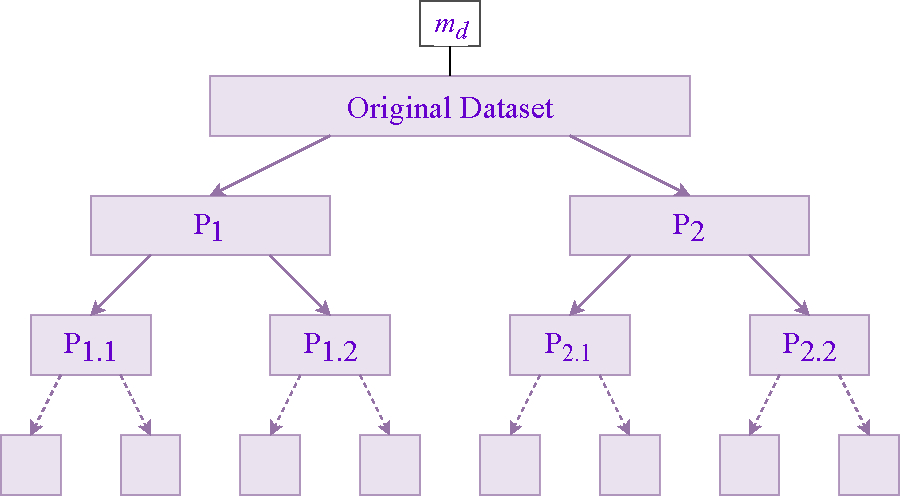
\includegraphics[width=0.7\linewidth]{figures/dnc-partitioning}
\caption{DNC Partitioning Process}
\label{fig:dnc-partitioning}
\end{figure}

When the recursive partitioning is completed, the resulting subsets get merged starting with the smallest ones. Whenever two partitions $P_{1}$ and $P_{2}$ are merged, the tuples in $P_{2}$ that are dominated by any tuple in $P_{1}$ are eliminated. The tuples in $P_{1}$ cannot be dominated by tuples from $P_{2}$, because they are \`{a}-priori better than the tuples in $P_{2}$ in at least one dimension, which is $d$. This is due to the division of the original dataset according to the median $m_{d}$. Hence, only incomparable tuples are left when the merging is complete. 
The merge process is illustrated in Fig.~\ref{fig:dnc-merging}. 

\begin{figure}[h]
\centering
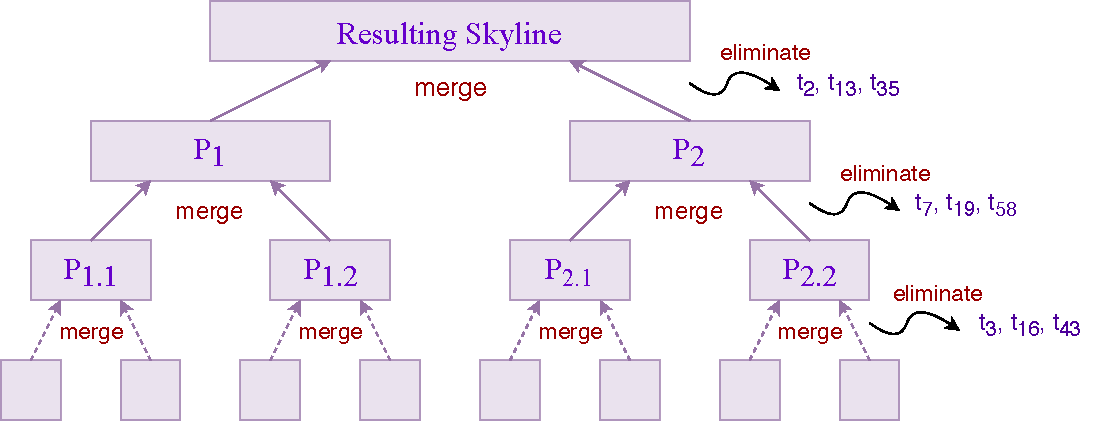
\includegraphics[width=0.9\linewidth]{figures/dnc-merging}
\caption{DNC Merging Process}
\label{fig:dnc-merging}
\end{figure}

Kossmann et al. \cite{kossmann} suggest to further improve the merging process by once again applying the divide-and-conquer principle. For this purpose, each of the two partitions $P_{1}$ and $P_{2}$ gets partitioned again; this time according to a different dimension ($d-1$ for instance). $P_{1}$ and $P_{2}$ are now split into $P_{1.1}$ and $P_{1.2}$, and $P_{2.1}$ and $P_{2.2}$, respectively. This has the advantage that not all tuples in $P_{1}$ and $P_{2}$ have to be compared to each other. Instead, now only the tuples in $P_{1.1}$ and $P_{2.1}$, in $P_{1.2}$ and $P_{2.2}$, and in $P_{1.1}$ and $P_{2.2}$ need to be compared. Thus, the step of comparing the tuples in $P_{1.2}$ to the tuples in $P_{2.1}$ can be omitted. This is because, due to the partitioning with the median $m_{d-1}$, the tuples in $P_{1.2}$ and in $P_{2.1}$ are incomparable. $P_{1.2}$ is better than $P_{2.1}$ in dimension $d$, and $P_{2.1}$ is better than $P_{1.2}$ in dimension $d-1$. The recursion of the merge function ends as soon as there are no unused dimensions left or the size of the respective subset is either 0 or 1. 
This advanced merging process is visualized in Fig.~\ref{fig:dnc-advanced-merge}. After the last two subsets have been merged, the resulting set of tuples is the skyline. 

The pseudo-code to the DNC algorithm is shown in Algorithm \ref{alg:dnc}. The C++ code, including the helper functions $merge$ and $partition$ can be found in Appendix \ref{appendix-code} to this work. 

\begin{figure}[h]
	\centering
	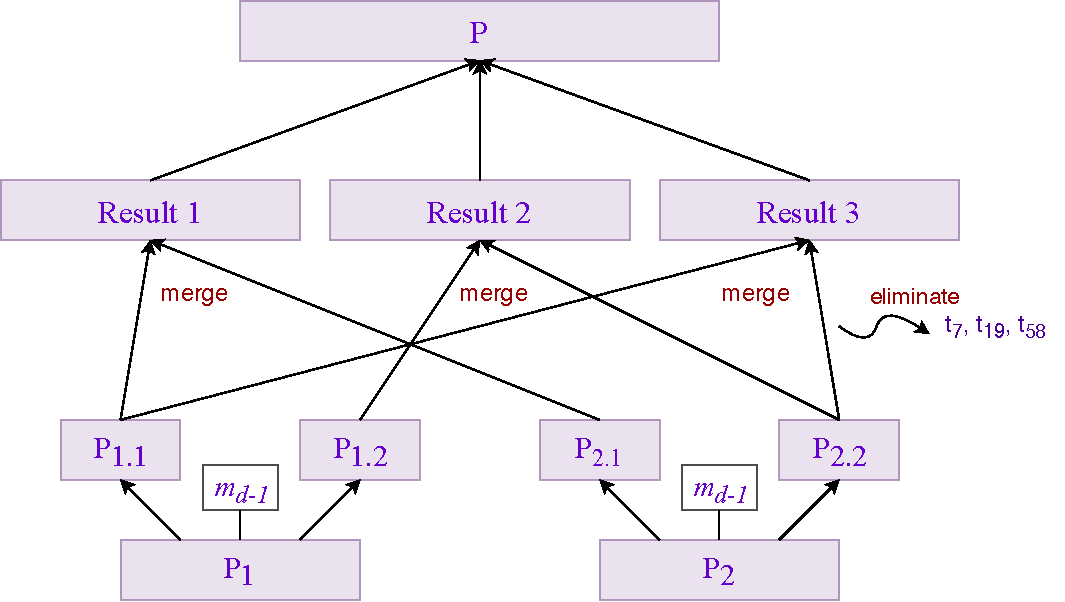
\includegraphics[width=0.9\linewidth]{figures/dnc-advanced-merge}
	\caption{DNC Advanced Merging}
	\label{fig:dnc-advanced-merge}
\end{figure}

% pseudo-code Divide-and-Conquer
\begin{algorithm}[h]
	\caption{Divide-and-Conquer Algorithm} \label{alg:dnc}
	\begin{algorithmic}[1] 
		\State \textbf{Input :} Tuple List $T$, Dimension $dim$
		\State \textbf{Output :} Skyline $skyline$
		\If {$T.size$ = 1} \textbf{return} $T$
		\EndIf
		\State $pivot \gets median$($T$, $dim$)
		\State ($P_{1},~P_{2}$) = $partition$($T$, $dim$, $pivot$)
		\State $S_{1} \gets$ Skyline($P_{1},~dim$)
		\State $S_{2} \gets$ Skyline($P_{2},~dim$)
		\State $merge\_result$ = $merge$($S_{1},~S_{2},~dim$)
		\State Add $S_{1}$ to $skyline$
		\State Add $merge\_result$ to $skyline$
		\State \textbf{return} $skyline$
	\end{algorithmic}
\end{algorithm}

% mway modification
For databases with limited main memory capacities the authors further suggest a modification to the basic DNC algorithm called \textit{M-way partitioning}. The main idea is to always partition the dataset in $M$ subsets instead of only two. $M$ should be chosen so that the size of the resulting partitions is small enough to fit into main memory. This approach has to be applied both during the partitioning phase as well as during the merging phase of the algorithm. This sort of modification, however, is not subject of this paper due to the context of in-memory databases. The M-way partitioning can be read up in more detail in \cite{kossmann}. 

%* DNC's worst-case complexity equals its best-case complexity\footnote{Which is $O(n~*~(log~n)^{d-2})~+~O(n~*~log~n)$.}~\cite{kossmann}. Therefore, the algorithm should only be taken in consideration when a high amount of ``worst-case scenarios'' is anticipated. 
Just like the BNL algorithm, Divide-and-Conquer cannot produce its results progressively, meaning that it can only output any of the skyline tuples, once the entire computation of the skyline is completed~\cite{survey}. 

\subsection{Other Algorithms}
With BNL and DNC being two of the more basic algorithms, several of the later proposed approaches reuse and extend their ideas, while optimizing the computation in specific areas. In the following, some of the newer skyline algorithms will be briefly introduced. 

% Bitmap, Index(index-based)
\subsubsection{Bitmap and Index Algorithms} \label{subsection:bitmap-index}
Bitmap \cite{bitmap-index} and Index \cite{bitmap-index} are two different algorithms aimed at producing the skyline tuples progressively while keeping response times generally low. 
The main idea of the Bitmap algorithm is to encode the underlying dataset as a bitmap structure in order to speed up computation \cite{survey}. In particular, the fact that bitwise operations are generally fast is exploited. At the beginning of the algorithm every single tuple from the underlying dataset has its attributes mapped into a bit-vector. Later, during computation, all comparison operations are executed on bit-slices derived from the bit-vectors. This enables the algorithm to quickly determine which tuples are dominated by others and which are not. 

The Index algorithm takes a different approach at progressive skyline computation and makes use of an index structure, namely a B$^{+}$-tree~\cite{bitmap-index}. In addition to that, while it does produce the skyline tuples progressively, it does not do so one-by-one, but does it in blocks instead~\cite{survey}. First, the algorithm implements a transformation mechanism which maps each tuple into one-dimensional space and stores it in the B$^{+}$-tree. During this process, tuples that are mapped to the same value are all stored in the same cluster. Due to the now existing sort order, the algorithm can decide which of the existing tuples are more likely to be part of the skyline, and therefore also behave more dominantly when eliminating other tuples. Also, tuples with common features that were previously mapped to land in the same cluster, can be checked for being part of the skyline in burst-like batches, which speeds up the performance and enables the algorithm to work progressively. 

% Nearest neighbor (NN), BBS (both with R* trees) both index-based
\subsubsection{NN and BBS Algorithms} \label{subsection:nn-bbs}
Another algorithm which is more focused on the ``big picture'' instead of the entire skyline, is the NN algorithm \cite{nn}. It is based on nearest-neighbor-search, hence the name. All the tuples of a dataset can be represented as $d$-dimensional points in a $d$-dimensional coordinate system. Assuming that the tuple attributes need to be minimized, the algorithm starts by applying nearest neighbor search to find the point that is closest to the origin. This point is inserted into the skyline right away. At this stage of the algorithm, it partitions the $d$-dimensional space of the coordinate system into four different partitions. The first one is the partition between the first point and the origin. It does not contain any further skyline points, as there are --- by definition of the nearest-neighbor-search --- no other points between the first one found and the origin. The second partition cannot contain any skyline points either, because they all have greater attribute values in every dimension than the first point, and are therefore dominated by it. The two remaining partitions can still contain points that are part of the skyline. The NN algorithm is recursively applied to these partitions for as long as there are any that are not empty. 

The nearest-neighbor-search component of the algorithm performs particularly well if the original dataset is indexed with a data structure such as the R*-tree. Just like the Bitmap and Index algorithms, the NN algorithm produces the skyline results progressively, i.e. without the need for the entire skyline to be computed before the first results are produced. While the first skyline tuples are output very fast, the rest of the skyline might need a much longer time to be computed \cite{nn}. 

A successor to the original NN algorithm, called BBS (Branch-and-Bound Skyline) \cite{bbs}, has been developed soon after. While it also makes use of the nearest-neighbor-search and the R*-tree, it has some significant improvements over the NN algorithm. One of these is that it only traverses the R*-tree once and thus reduces the number of redundant accesses. The algorithm organizes all of the skyline candidates in a heap and keeps them sorted according to their minimal distance from the origin \cite{survey}. There is more information on the BBS algorithm given in \cite{bbs}. 
%The first heap entry is the root of the R*-tree. In each iteration, the algorithm removes the entry at the top of the heap and does one of the following: 
%\begin{itemize}
%	\item If the removed heap entry is an inner node, then its not-dominated children are added to the heap and the next iteration of the algorithm starts. 
%	\item If the removed heap entry is a leaf node, then it is tested for being dominated, and if not inserted into the skyline.
%\end{itemize}

% Sort-filter-skyline (SFS) - sorting based BNL, Less is pretty similar, both sort-based
\subsubsection{Sorting-Based Algorithms} \label{subsection:sorting-based-algorithms}
There exists an entire range of sorting-based algorithms for skyline computation. The somewhat earlier developed SFS algorithm (Sort-Filter-Skyline) \cite{sfs} reuses the idea of the BNL algorithm and adjusts it so that the tuples are no longer considered in arbitrary order, but are instead presorted first. Then the tuples that are more likely to be part of the skyline are read in first. This way, the skyline can be computed faster, as the tuples inserted into the skyline at the beginning are very likely to be efficient ``tuple-killers'' and to eliminate most of the dominated tuples very fast. In addition to that, eligible tuples can be output progressively, which was not originally the case with the BNL algorithm. The drawback of presorting the underlying dataset is usually well compensated by the significantly reduced number of comparisons. 

% Less is too complex for such a minor improvement to list it here
%Another algorithm that shares its roots with BNL is LESS (Linear Elimination Sort for Skyline)(ref less). Just like the SFS algorithm, it presorts the original dataset, preferably with a special entropy scoring function. The authors suggest to hold an \textit{elimination filter} window with the most dominant tuples during the first pass of the external sorting function. This enables to discard dominated tuples fairly quickly. 

% SaLSa - based on SFS and LESS, direct predecessor of ST-S, sort-based
A further improvement over the SFS algorithm is its successor SaLSa (Sort and Limit Skyline Algorithm) \cite{salsa}. Just like SFS, it presorts the original dataset. However, this does not only happen for the reason of reducing the entire number of comparisons during computation. The key idea of SaLSa is to implement a threshold mechanism to stop the algorithm early as soon as all the tuples left are dominated by the tuples already in the skyline. In order to enable this technique, a slightly different sorting function is suggested, which works as following: First, all the tuples are presorted (ascending) according to their smallest attribute value among all dimensions. Then, if two or more tuples compete for the same position in the sorted set, the one with the smaller sum of attribute values across all dimensions wins the tie and gets the lesser position in the set. 

Later, during each iteration of the algorithm, the threshold value is updated with respect to the newest tuple that was read in. As soon as the stopping condition is reached, all tuples that are left, are dominated by the threshold, and the algorithm terminates. The stopping mechanism will be discussed in more detail in chapter \ref{subsection:sts}. 
Unfortunately, the threshold only reduces the number of tuples processed by the algorithm, but is not as efficient in scenarios with high dimensionality \cite{survey}. 

\subsection{ST-S Algorithm} \label{subsection:sts}
%introduction
One of the newest skyline algorithms to date is the ST-S (Skyline using Tree Sorting-based) algorithm \cite{rahman}. It is based on SaLSa, which, in its turn, is based on BNL and SFS. Thus, ST-S also belongs to the ``family'' of sorting-based algorithms. Its main addition to the concept of SaLSa is an algorithm-internal indexing structure, which is similar to a radix tree. This special tree structure is called \textit{N-Tree} within this work. The main purpose of the N-Tree is to execute dominance checks much faster by reducing the overall amount of comparisons between tuples. There are two drawbacks to the tree-based dominance checks. The first one is that ST-S is only suitable for categorical attributes, because continuous attributes (e.g. \textit{double} values) would imply an almost infinite amount of possible categories, and thus far too many children for each of the inner nodes of the tree. The second disadvantage is the somewhat higher memory usage during computation, as the tree structure takes up some of the available space. Using a tree structure to store skyline candidates however means that no separate \textit{window}, like in the original BNL algorithm, is needed. The authors in \cite{rahman} claim that ST-S significantly outperforms its predecessor SaLSa for categorical attributes in terms of computation time. In chapter \ref{chapter:Evaluation} of this work, ST-S will be further compared to the Naive-Nested-Loops and SARTS algorithms. 

%algorithm explanation
While the authors of the original paper \cite{rahman} work with binary attribute values (i.e. each attribute is either 0 or 1), they also propose using more categories if needed in a specific use case. This paper makes use of this proposition for generality purposes and implements the tree variant with multiple possible categories. 
The resulting tree structure used in ST-S is shown in Fig.~\ref{fig:ntree}. Every inner node, including the root, has an array which can hold as many children as there are possible attribute values. Hence, if all the values in the set $S := \{0,~1,~2,~3,~4\}$ can be taken, then each of the tree nodes has an array of size $|S| = 5$ with up to 5 different children. Each path taken from the root to a leaf represents the assignment of attribute values of some particular inserted tuple(s). The IDs of the tuples are always saved in form of arrays within the leaves. In addition to that, each of the inner nodes contains two different score values --- a \textit{minScore} and a \textit{maxScore}. MinScore represents the smallest possible score that can be achieved within leaves reachable from the current node. MaxScore stores the highest possible score, respectively. An illustration of the nodes is given in Fig.~\ref{fig:nnode}. 

\begin{figure}[h]
	\centering
	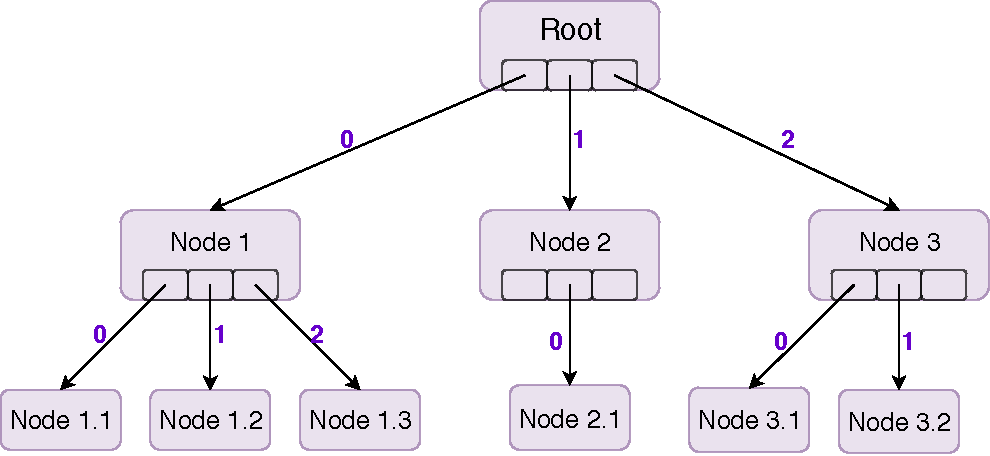
\includegraphics[width=0.8\linewidth]{figures/ntree}
	\caption{N-Tree for ST-S Algorithm}
	\label{fig:ntree}
\end{figure}

\begin{figure}[h]
	\centering
	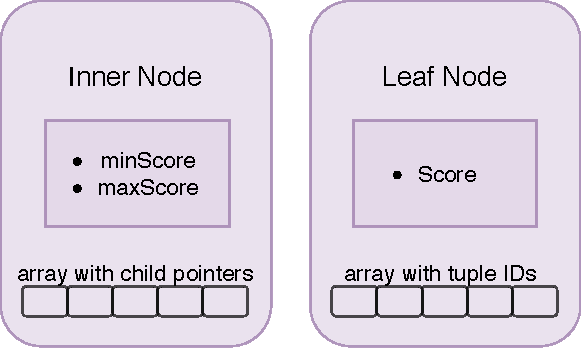
\includegraphics[height=0.3\linewidth]{figures/nnode}
	\caption{Nodes of the N-Tree}
	\label{fig:nnode}
\end{figure}

The score of a particular tuple is determined by a scoring function, let us call it $F$. The only condition that $F$ must fulfill is to not assign a higher score to a tuple that is dominated than to its dominator. The scoring function used in the following is 
\begin{equation}
F(t)~:=~\sum_{i~=~0}^{n-1}(2^{n~-~i}~*~t[A_{i}]), 
\end{equation}
with $t$ being the tuple to receive a score, $n$ the length of the tuple, and $t[A_{i}]$ the $i$-th attribute of the tuple. 

At the beginning, the tuples are sorted with the monotonic function \textit{minC()} (resp. \textit{maxC()} if the attributes have to be maximized). \textit{minC()} is defined as 
\begin{equation}
minC(t) := (min_{A_{i}}\{t[A_{i}]\},~\sum_{A_{i}}(t[A_{i}])).
\end{equation}
It consists of two components as mentioned in chapter \ref{subsection:sorting-based-algorithms}: a main comparison attribute, which is the smallest of all attribute values of a tuple, and a tie-breaker being the sum over all attribute values of the same tuple. Suppose the dataset shown in Fig.~\ref{fig:minc}~(a). By applying the sorting function \textit{minC} to the dataset, the sorted list of tuples shown in Fig.~\ref{fig:minc}~(b) emerges. 

\begin{figure}[h]
	\centering
	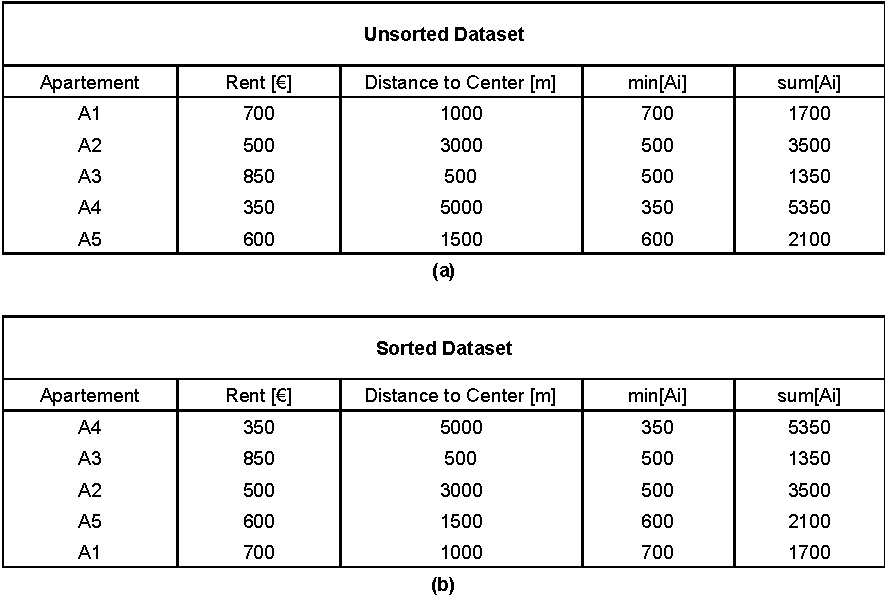
\includegraphics[width=0.95\linewidth]{figures/minc}
	\caption{Example: Sorting with \textit{minC()}}
	\label{fig:minc}
\end{figure}

The pseudo-code to the ST-S algorithm is given in Algorithm \ref{alg:sts}. It works as following: 
\begin{enumerate}
	\item The tuples are presorted with \textit{minC()} (line 3).
	\item $t_{stop}$ is the threshold, and is undefined at the beginning. It is later updated (lines 13-14) with knowledge of some tuples that have been proved to be part of the skyline. 
	\item The first tuple $t_{0}$ from the presorted dataset is always part of the skyline due to the choice of \textit{minC()}. It gets inserted into the tree and is put out as part of the skyline (lines 5-7). 
	\item In the following loop every tuple $t$ of the sorted dataset, except for the first one $t_{0}$, is checked for being dominated by any tuple already in the skyline (line 10). The checks are carried out with the help of the tree, which holds all the skyline tuples to date. The responsible operation \textit{is\_dominated} will be introduced in more detail later. 
	\item If a tuple $t$ is dominated by some other tuple in the skyline, it is no longer considered for the skyline. If it is not dominated, it gets inserted into the tree (line 11), so that it is able to eliminate future tuples that are not part of the skyline. 
	\item If the maximum attribute value of the new skyline tuple $t$ is smaller than the maximum attribute value of the threshold $t_{stop}$, then the threshold is updated (line 14), and now holds the value of $t$, until the next update occurs. 
	\item At the beginning of each iteration of the loop, the stopping condition is checked (line 9), so that the algorithm can stop early if all the tuples left in the dataset are \`{a}-priori dominated by the threshold. This functionality has been inherited from the SaLSa algorithm (chapter \ref{subsection:sorting-based-algorithms}). If the maximum attribute value of the threshold tuple $t_{stop}$ is less or equal to the minimum attribute value of the current tuple $t$, and the two tuples are not the same, then thanks to presorting with \textit{minC()} none of the remaining tuples can be part of the skyline. At this point, the algorithm can terminate and the tree with the tuples is no longer needed. If the tuples are the same, however, then the current tuple also has to be checked to be part of the skyline. 
\end{enumerate}

% pseudo-code ST-S
\begin{algorithm}[h]
	\caption{ST-S Algorithm} \label{alg:sts}
	\begin{algorithmic}[1] 
		\State \textbf{Input :} Tuple List $T$, Tree $tree$
		\State \textbf{Output :} Skyline $skyline$
		\State Sort $ T $ in-place using a monotonic function \textit{minC()}
		\State $t_{0} \gets $ first element of $T$
		\State $t_{stop} \gets t_{0}$
		\State insert($t_{0}$, $tree.root$, 0)
		\State Add $t_{0}$ to $skyline$ $~~~~~$ {\footnotesize // $t_{0}$ always part of skyline due to presorting}
		\For {each tuple $t~\in~T\backslash\{t_{0}\}$}
			\If {$max$($t_{stop}$)$~\leq~min$($t$) and $t_{stop}~\neq~t$}
				\textbf{return}
			\EndIf
			\If {\textbf{not} is\_dominated($t$, $tree.root$, 0, $score(t)$)}
				\State insert($t$, $tree.root$, 0)
				\State Add $t$ to $skyline$
				\If {$max(t)~<~max(t_{stop})$}
					\State $t_{stop} \gets t$ 
				\EndIf
			\EndIf
		\EndFor	
	\end{algorithmic}
\end{algorithm}

\noindent Both the \textit{insert} and \textit{is\_dominated} operations have been slightly modified from the original variant, in order to incorporate multiple attribute categories instead of just two. They also make use of the \textit{minScore} and \textit{maxScore} functionality to speed up dominance checks within the tree. 

The pseudo-code to the \textit{insert} operation is shown in Algorithm \ref{alg:sts-insert}. The proceedings are the following: 
\begin{enumerate}
	\item Depending on the current depth level within the tree, the \textit{minScore} and \textit{maxScore} attributes of the current node are updated (lines 2-7). On level 0 (root level) the smallest possible score is 0, and the highest possible score is calculated using the greatest-possible attribute value for each of the remaining levels. If the current node is not the root, the scores are updated by applying the scoring function in accordance with the current tree level and the attribute values which already occured. 
	\item If the current level is the deepest level possible, then it means that the algorithm reached a leaf node (line 8). At this point, if some other tuple has already been inserted in this leaf node, the score of the leaf no longer needs to be calculated. If the current tuple is the first one to get stored in the leaf, then the node's score is updated. In any case, the \textit{tupleID} of the tuple is attached to the \textit{tupleIDs} list of the leaf node (lines 9-10). 
	\item If the last level has not yet been reached, then the tree has to be further traversed. For this purpose, the \textit{insert} operation is called recursively on the child node at position $t[level]$ with the same tuple $t$ and the \textit{level} increased by one (line 15). 
	\item If the child at the position $t[level]$ does not yet exist, it is simply created as a new node (lines 13-14) before further traversing the tree. 
\end{enumerate}

% pseudo-code INSERT
\begin{algorithm}[h]
	\caption{INSERT Operation for ST-S} \label{alg:sts-insert}
	\begin{algorithmic}[1]		
		\State \textbf{Input :} Tuple $t$, Node $node$, Level $level$, Attributes $atts$
		\If {$level$ = 0}
			\State $node.minScore \gets 0$
			\State $node.maxScore \gets \sum_{i~=~0}^{t.size~-~1}(2^{t.size~-~i}~*~max(atts))$
		\Else 
			\State $node.minScore \gets \sum_{i~=~0}^{level~-~1}(2^{t.size~-~i}~*~t[i])$
			\State $node.maxScore \gets node.minScore~+~\sum_{i~=~level}^{t.size~-~1}(2^{t.size~-~i}~*~max(atts))$
		\EndIf
		\If {$level$ = $t.size$} 
			\If {$node.score$ is $None$}
				\State $node.score \gets score(t)$
			\EndIf
			\State Append $t.tupleID$ to $node.tupleIDs$
		\Else
			\If {$node.child[t[level]]$ \textbf{not} exists}
				\State $node.child[t[level]] \gets New$ Node()
			\EndIf
			\State insert($t$, $node.child[t[level]]$, $level~+~1$)
		\EndIf
	\end{algorithmic}
\end{algorithm}

\noindent The pseudo-code to the \textit{is\_dominated} operation can be seen in Algorithm \ref{alg:sts-is-dominated}. Starting from the root, the tree is traversed from top to bottom. The usage of the sorting and scoring functions enables the algorithm to only search in those branches of the tree that are not \`{a}-priori dominated. 
\begin{enumerate}
	\item In this work the wish to minimize the attribute values is assumed. Therefore, only those children of the current node that have a smaller position than $t[level]$ are further considered in the dominance test. These children are recursively traversed by the \textit{is\_dominated} function (lines 7-11). 
	\item If the current node is \textit{None}, then it has not yet been initialized, and thus also does not have any children that the algorithm could traverse. Hence, there are no paths from the current node that would dominate the given tuple. \textit{False} is returned (line 3). 
	\item Also, if the score of the given tuple is smaller than the smallest-possible score of the current node, then, due to our choice of the scoring function, the tuple cannot be dominated by any path through this node. \textit{False} is returned (line 3). 
	\item If by traversing the tree the deepest possible \textit{level} has been reached, the algorithm checks whether the score of the given tuple equals the score of the leaf node. If the scores are equal, then the tuple is obviously not dominated by the other tuples in this leaf node, and \textit{False} is returned (line 5). Otherwise, \textit{True} is returned and the tuple is no longer considered a skyline candidate (line 6). 
\end{enumerate}

% pseudo-code IS_DOMINATED
\begin{algorithm}[]
	\caption{IS\_DOMINATED Operation for ST-S} \label{alg:sts-is-dominated}
	\begin{algorithmic}[1]		
		\State \textbf{Input :} Tuple $t$, Node $node$, Level $level$, Score $s$
		\State \textbf{Output :} True if $t$ is dominated, otherwise False
		\If {$node$ is $None$ or $s < node.minScore$} \textbf{return} False
		\EndIf
		\If {$level = t.size$ and $score(t)~\neq~node.score$} \textbf{return} True
		\EndIf
		\If {$level = t.size$ and $score(t)~=~node.score$} \textbf{return} False
		\EndIf
		\State $weight \gets 2^{t.size~-~level}~*~t[level]$
		\For {each $i~\in~N_{0},~i~<~t[level]$}
			\If {is\_dominated($t$, $node.child[i]$, $level~+~1$, $s~+~weight$)}
			\State \textbf{return} True
			\EndIf
		\EndFor
		\If {is\_dominated($t$, $node.child[t[level]]$, $level~+~1$, $s$)}
		\State \textbf{return} True
		\EndIf
		\State \textbf{return} False
	\end{algorithmic}
\end{algorithm}

% If not enough content, also cover ST-P and TA-SKY

\subsection{Classification} \label{classification}
The previously introduced skyline algorithms can be organized according to different criteria. %, such as their basic idea, the algorithms they are related to, as well as whether they can produce results progressively or not \cite{survey}. 
A classification with criteria related to the topic of this work is given in Table~\ref{fig:classification}. 

\begin{figure}[h]
	\centering
	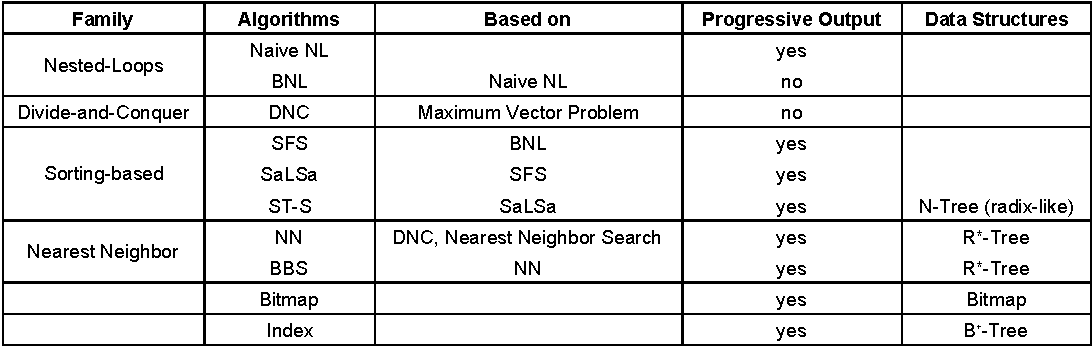
\includegraphics[width=1\linewidth]{figures/classification}
	\captionof{table}{Classification of Introduced Algorithms}
	\label{fig:classification}
\end{figure}

\subsection{Parallelization Approaches} \label{subsection:parallelization-approaches}
%While applications can generally be parallelized with the help of GPUs, multicore CPUs, as well as in distributed environments, such as MapReduce \cite{book-kemper}, 
The focus of this work lies within multicore parallelization with CPUs. In the following, some of the modern approaches to parallelization of skyline algorithms are briefly covered. 

\subsubsection{Parallelization Criteria} \label{subsection:parallelization-criteria}
Chester et al. \cite{chester} (2015) propose in their work on skyline parallelism the main criteria for developing efficient multicore parallelization approaches. The key suggestions are: 
\begin{enumerate}
	\item When dividing the input data into subsets, the resulting data blocks should be independent, unordered, and about equal-sized. This way, the results of each working unit will not depend on the results of other units and the workload will be close to equally distributed. 
	\item Data structures that are shared between threads should be either in read-only mode, or only have a few write changes during parallelization. While the coordination on write accesses could be achieved by locking, this often results in a major bottleneck of the otherwise parallel execution. If the number of writes is high and no locks are used, race conditions between threads are almost certain to occur. 
	\item If synchronization points are used, their location in the code should be chosen very carefully. At these points, there is no parallel processing both during the time of waiting for the single threads to finish their current work, and during the time of sequential synchronization. If the synchronization points were chosen wrongly, the performance of the algorithm will most certainly take a significant hit. 
\end{enumerate}

%\subsubsection{Parallelizing BBS} \label{subsection:parallelizing-bbs}
%Park et al. \cite{parallel-bbs} (2011) made successful use of \textit{skeletal parallel programming} \cite{skeletal} when parallelizing the previously mentioned BBS algorithm (chapter \ref{subsection:nn-bbs}). 
%For this purpose the authors used the OpenMP~\cite{openmp} parallelization framework, which parallelizes given regions of the program by issuing compiler directives. Parallelization with OpenMP is usually relatively well applicable to already existing sequential programs, as adding compiler directives to parallelizable regions of the code usually does not imply any significant code changes. For a naive parallelization approach, Park et al. identified the two most computation-intensive parts of the program and simply annotated them with OpenMP parallelization directives. However, this did not produce the desired speedup of the algorithm. The reason for this was that the parallel-running threads are not per-se able to exchange information on already eliminated tuples and thus the entire number of comparisons per skyline significantly rises. OpenMP does not allow the programmer to stop threads by \textit{break} command or equals during runtime\footnote{I.e. it issues compilation errors. This was checked in the scope of this work.}. Enabling explicit communication patterns between threads would slow the program down significantly as explained earlier in this chapter. 
%
%% TODO right now the solution doesnt make too much sense
%The solution was to first gather the incomparable candidate tuples, and afterwards to inspect these in parallel using \textit{tbb's parallel\_for}~\cite{parallel-for} construct. 
%This paper will further consider OpenMP and tbb's parallel\_for as parallelization frameworks for the relevant skyline algorithms (chapter \ref{chapter:Parallelization}). 

% specially developed parallel skyline algorithms
\subsubsection{Existing Parallel Algorithms} \label{subsection:other-parallel-algorithms}
%Only a few of the existing sequential algorithms have been parallelized so far. One of these is the previously mentioned BBS algorithm for instance. In their work, Park et al. made successful use of \textit{tbb's parallel\_for}~\cite{parallel-for} construct after identifying the regions in their code suitable for parallelization \cite{parallel-bbs}. Their first attempt to parallelize the critical regions with OpenMP~\cite{openmp}, however, failed as the parallelization was not able to improve the computation time of the initial algorithm. In this work, OpenMP and tbb's parallel\_for will be further considered as parallelization frameworks for the relevant skyline algorithms. 

A range of new algorithms, specifically developed for parallel execution, has recently appeared. Some of the interesting ones to read up on include \textit{pskyline}~\cite{parallel-bbs} and \textit{APSkyline}~\cite{apskyline} based on the divide-and-conquer principle, \textit{Hybrid}~\cite{chester} making use of prefiltering, partitioning, and sorting, \textit{SkyAlign}~\cite{skyalign}, which is one of the few skyline algorithms specifically designed for GPU computation, as well as \textit{MR-GPMRS} \cite{map-reduce} designed for computation with the MapReduce paradigm. This paper will not discuss these algorithms in greater detail, as it is more aimed at parallelizing existing sequential algorithms, as well as the novel SARTS algorithm (chapter \ref{chapter:ARTforSkyline}). 




%One of the main achievements of Kung et al. was probably to determine the theoretically applicable upper bounds for the number of comparisons a skyline algorithm might have to perform. These boundaries apply to the worst-case scenario. With $C_{max}$ being the maximum number of comparisons, $n$ the number of vectors, and $dim$ the number of dimensions of each vector, according to Kung et al. we receive: 
%\begin{equation}
%C_{max}(n) = n - 1 for dim = 1, 
%\end{equation}
%\begin{equation}
%C_{max}(n) \leq O(n log n) for dim = 2,3,  
%\end{equation}
%\begin{equation}
%C_{max}(n) \leq O(n (log n)^{d-2}) for dim \geq 4, 
%\end{equation}

